\documentclass[book]{jlreq}

\usepackage{graphicx}
\usepackage{amsmath,amssymb,amsthm}
%\usepackage{mathtools}
%%\usepackage{siunitx}
\usepackage{physics}
\usepackage{bm}

\renewcommand{\today}{\the\year/\the\month/\the\day}
\renewcommand{\contentsname}{Contents}
\renewcommand{\refname}{References}
\renewcommand{\figurename}{Fig.~}
\renewcommand{\tablename}{Table~}

\begin{document}
\title{Beam Loading}
\author{Shin-ichi YOSHIMOTO}
\maketitle
\tableofcontents
%%\clearpage

\part{数学的基礎}
\chapter{フーリエ変換とラプラス変換}
\section{周波数伝達関数}

時間領域における畳み込み積分
%
\begin{equation}
    y(t) = g(t)*x(t) = \int_0^{\infty} g(\tau) x(t - \tau) d\tau
\end{equation}
%
をフーリエ変換すると、
%
\begin{equation}
    Y(j\omega) = G(j\omega) X(j\omega)
\end{equation}
%
ただし、
%
\begin{equation}
    \begin{split}
        X(j\omega) = \int_{-\infty}^{\infty} x(t) e^{j\omega t} dt \\
        Y(j\omega) = \int_{-\infty}^{\infty} y(t) e^{j\omega t} dt \\
        G(j\omega) = \int_{-\infty}^{\infty} g(t) e^{j\omega t} dt
    \end{split}
\end{equation}

\part{Beam Loading}
\chapter{Static Beam Loading}
\section{Cavityの基礎}
\subsection{Power dissipation}
\begin{equation}
    P_{diss} = \frac{1}{2} \cdot \frac{V_{cav}^2}{R} = \frac{V_{cav}^2}{R_{sh}} 
\end{equation}

\subsection{Shut impedance}
\begin{equation}
    R = \frac{1}{2}\cdot R_{sh}
\end{equation}

空洞の入力カップラーの変圧比を$1:n$とすると(Fig. \ref{fig:Ideal_Trans})、
%
\begin{figure}[hbt]
    \begin{center}
        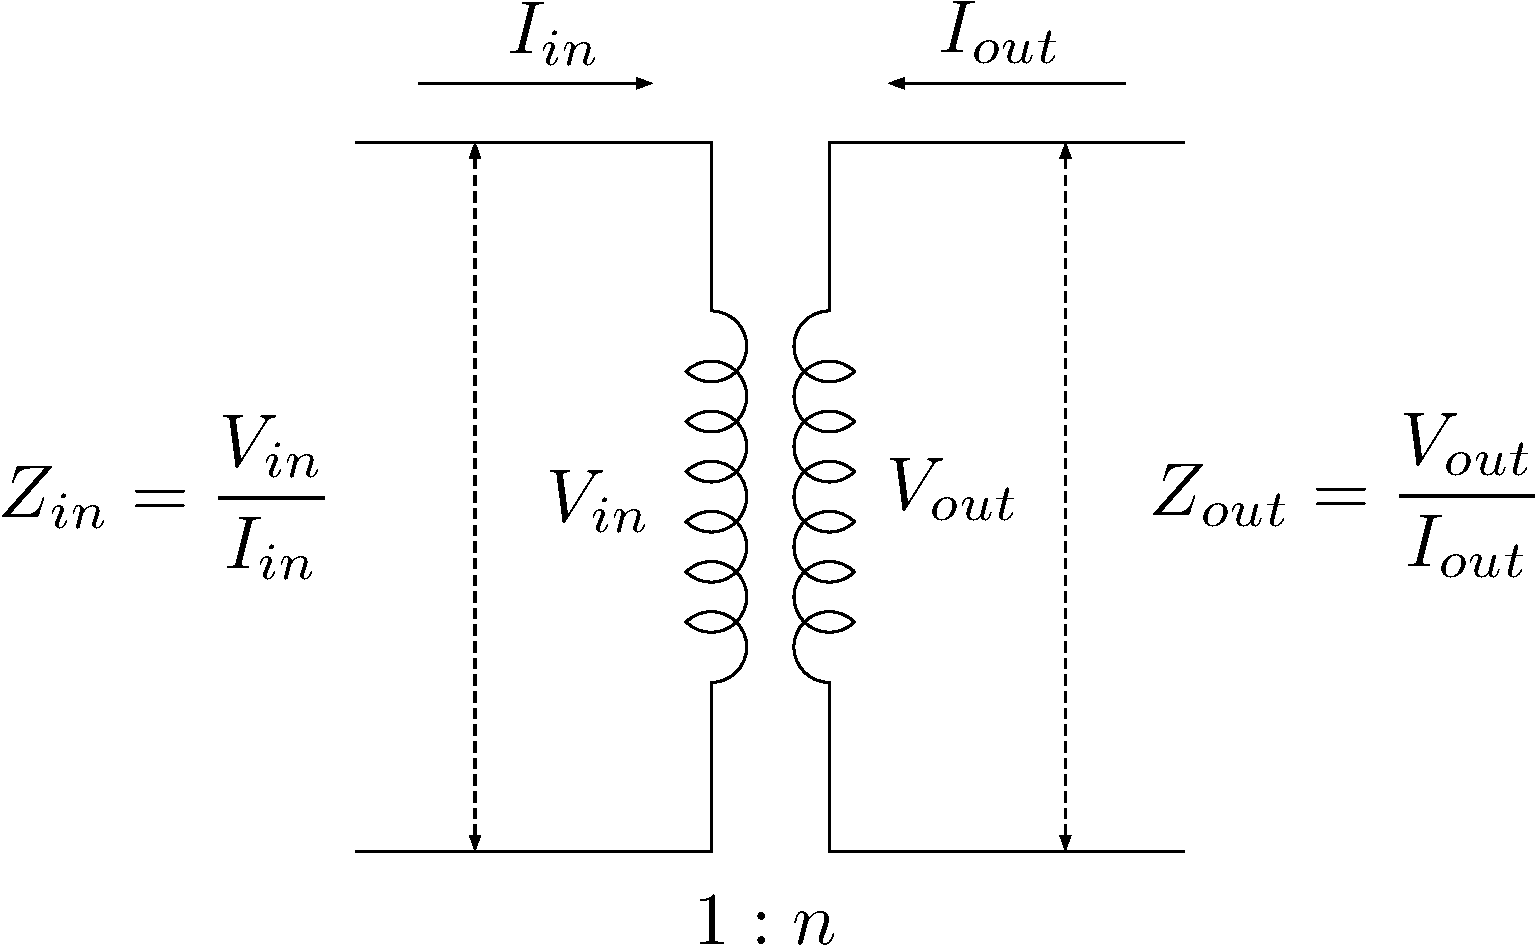
\includegraphics[width=12cm,clip]{figs/Ideal_Transformer.pdf}
        \caption{理想的なトランスによる入力カップラー.}
        \label{fig:Ideal_Trans}
    \end{center}
\end{figure}
%
\begin{equation}
    V_2 = N\cdot V_1, \; I_2 = \frac{1}{N}\cdot I_1
\end{equation}
%
したがって、
\begin{equation}
    Z_2 = n^2 \cdot Z_1 
\end{equation}


\section{ビーム負荷付き空洞のRCL等価回路}

\begin{figure}[hbt]
    \begin{center}
      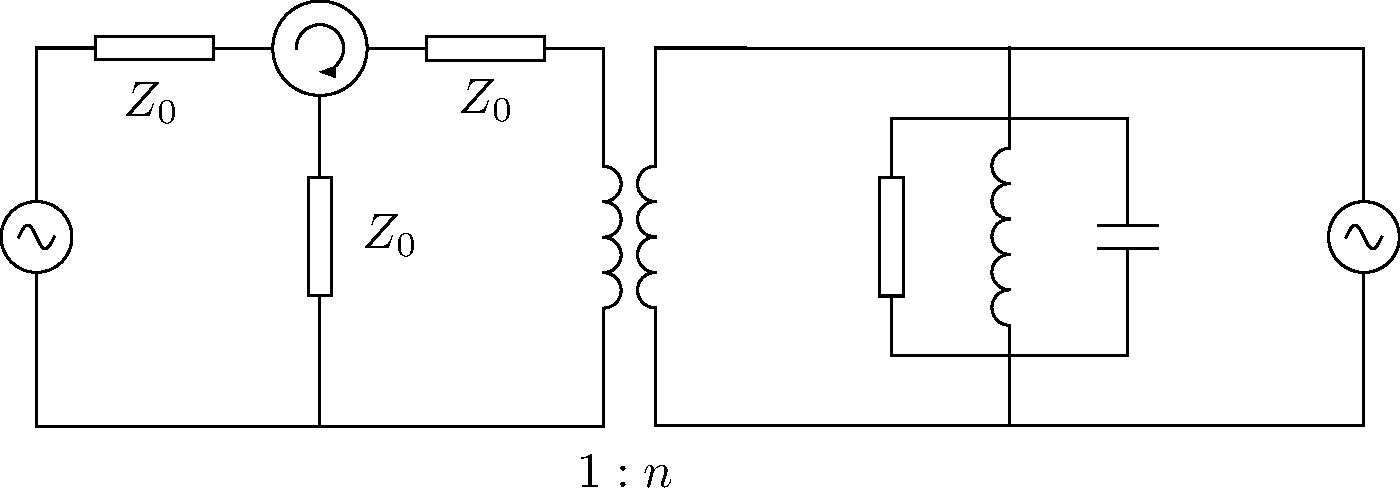
\includegraphics[width=12cm,clip]{figs/Cavity_Model.pdf}
      \caption{理想的なトランスによる入力カップラー.}
     \label{Cavity_Model}
    \end{center}
\end{figure}

\subsection{Cavity parameters}

\begin{figure}[hbt]
    \begin{center}
      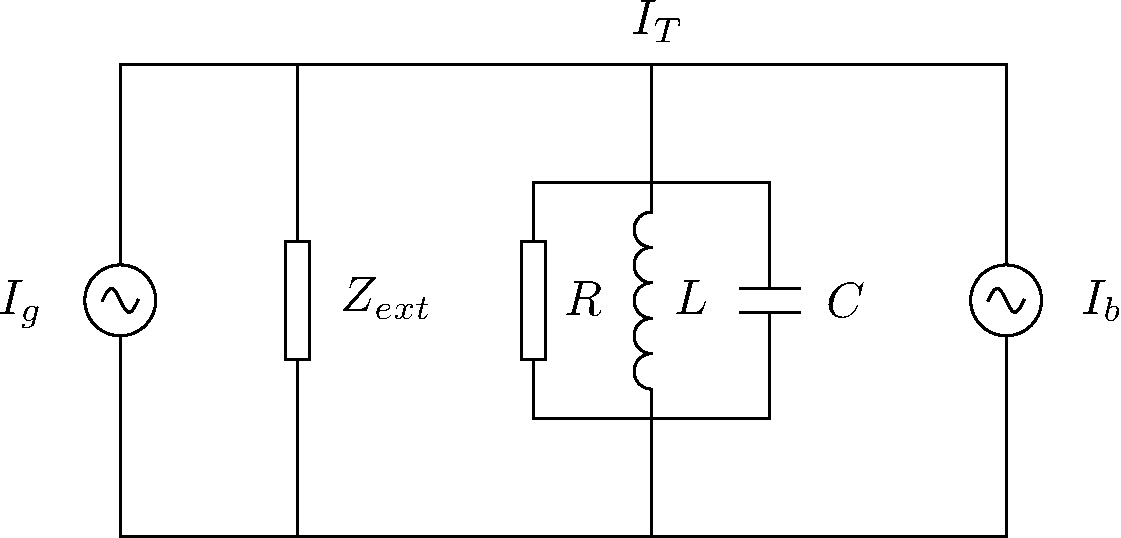
\includegraphics[width=12cm,clip]{figs/Equivalent_Circuit}
      \caption{等価回路}
     \label{Equivalent_Circuit}
    \end{center}
\end{figure}
%
\paragraph{共振周波数}
%
\begin{equation}
    \omega_0 = \frac{1}{L C}
\end{equation}
%
\paragraph{Quality factor}
%
\begin{equation}
    Q = 2\pi \frac{\mathrm{stored\;energy\;in\;cavity}}{\mathrm{dissipated \; energy\;per\;cycle}} = \frac{\omega_0 W}{P_{diss}}
\end{equation}
%
\paragraph{Unloaded quality factor}
%
\begin{equation}
    Q_0 = \omega_0 \frac{(1/2) C V^2}{V^2/(2R)} = \omega_0 R C 
\end{equation}
%
\paragraph{External quality factor}
%
\begin{equation}
    Q_{ext} = 2\pi \frac{\mathrm{stored\;energy\;in\;cavity}}{\mathrm{dissipated \; energy\;in\;external\;devices\;per\;cycle}}
     = \frac{\omega_0 W}{P_{ext}}
\end{equation}
%
\paragraph{Loaded quality factor}
%
\begin{equation}
    Q_L = 2\pi \frac{\mathrm{stored\;energy\;in\;cavity}}{\mathrm{total \; energy\;per\;cycle}} = \frac{\omega_0 W}{P_{tot}}
\end{equation}
%
ここで、
%
\begin{equation}
    P_{tot} = P_{diss} + P_{ext}
\end{equation}
%
したがって、
%
\begin{equation}
    \frac{1}{Q_L} = \frac{1}{Q_0} + \frac{1}{Q_{ext}}
\end{equation}
%
\begin{equation}
    \frac{1}{R_L} = \frac{1}{R} + \frac{1}{Z_{ext}}
\end{equation}
%
\paragraph{Coupling factor \beta}
%
\begin{equation}
    \beta = \frac{P_{ext}}{P_{cav}} = \frac{Q_0}{Q_{ext}} = \frac{R}{Z_{ext}} = \frac{R}{n^2 Z_0}
\end{equation}
%
\begin{figure}[hbt]
    \begin{center}
      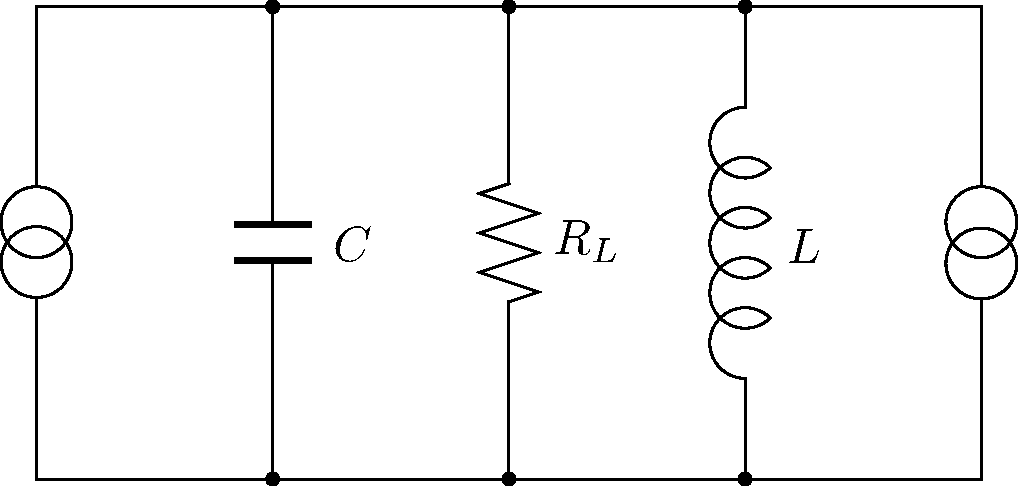
\includegraphics[width=12cm,clip]{figs/Equivalent_Circuit2}
      \caption{等価回路2}
     \label{Equivalent_Circuit2}
    \end{center}
\end{figure}
%
\begin{equation}
    \ddot{V}(t) + \frac{1}{R_L C}\dot{V}(t) + \frac{1}{L C} V(t) = \frac{1}{C} \dot{I}(t)
\end{equation}
%
\paragraph{Phasor}
\begin{equation}
    V(t) = \tilde{V}e^{j\omega_c t}, \; I(t) = \tilde{I}e^{j\omega_c t}
\end{equation}

\clearpage

\section{Pedersen Model \cite{Pedersen} \cite{Ninomiya}}

% \begin{figure}[hbt]
%     \begin{center}
%         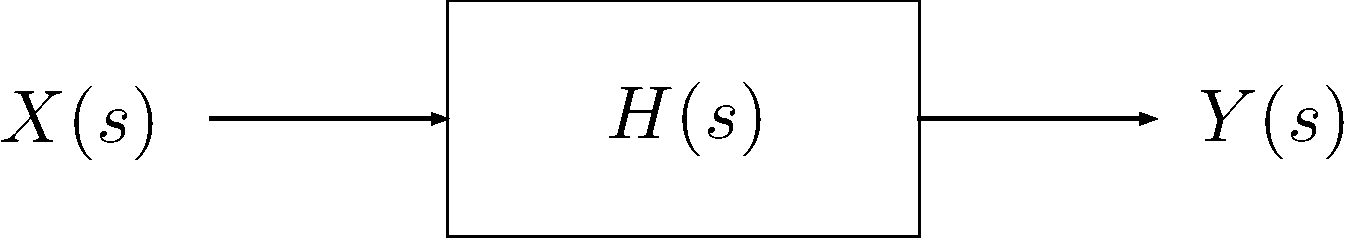
\includegraphics[width=12cm,clip]{figs/Transfer_Function.pdf}
%         \caption{伝達関数}
%         \label{fig:TF}
%     \end{center}
% \end{figure}

振幅変調$a(t)$や位相変調$\phi(t)$された正弦波信号を伝達関数$H(s)$を持つシステムに入力した場合,出力信号は一般に振幅変調と位相変調の両方を受けることになる。変調の振幅が十分小さい場合$(a \ll 1, \phi \ll 1)$の場合、変調の伝達は線形であり、以下のように決定される。

角振動数$\omega_c$の正弦搬送波を振幅を$a(t)$、位相を$\phi(t)$で変調した入力信号$x(t)$を


変調の伝達は、システムの伝達関数$Z(s)$から導き出すことができる。4つの変調伝達関数のセットを計算する必要があります。

システム解析には、このような変調が増幅器と空洞共振器を介して伝達されることを知ることが必要です。完全な特性評価には4つの異なる伝達関数が必要です。

低変調指数($a \ll 1, p \ll 1$)の場合、変調のトランスミッションは線形であり、次式で決定される。
%
\begin{enumerate}
    \item $G_{aa}(s)$ : 入力の振幅変調が出力の振幅を変調する伝達関数
    \item $G_{pp}(s)$ : 入力の位相変調が出力の位相を変調する伝達関数
    \item $G_{ap}(s)$ : 入力の振幅変調が出力の位相を変調する伝達関数
    \item $G_{pa}(s)$ : 入力の位相変量が出力の振幅を変調する伝達関数
\end{enumerate}
%
\begin{figure}[hbt]
    \begin{center}
        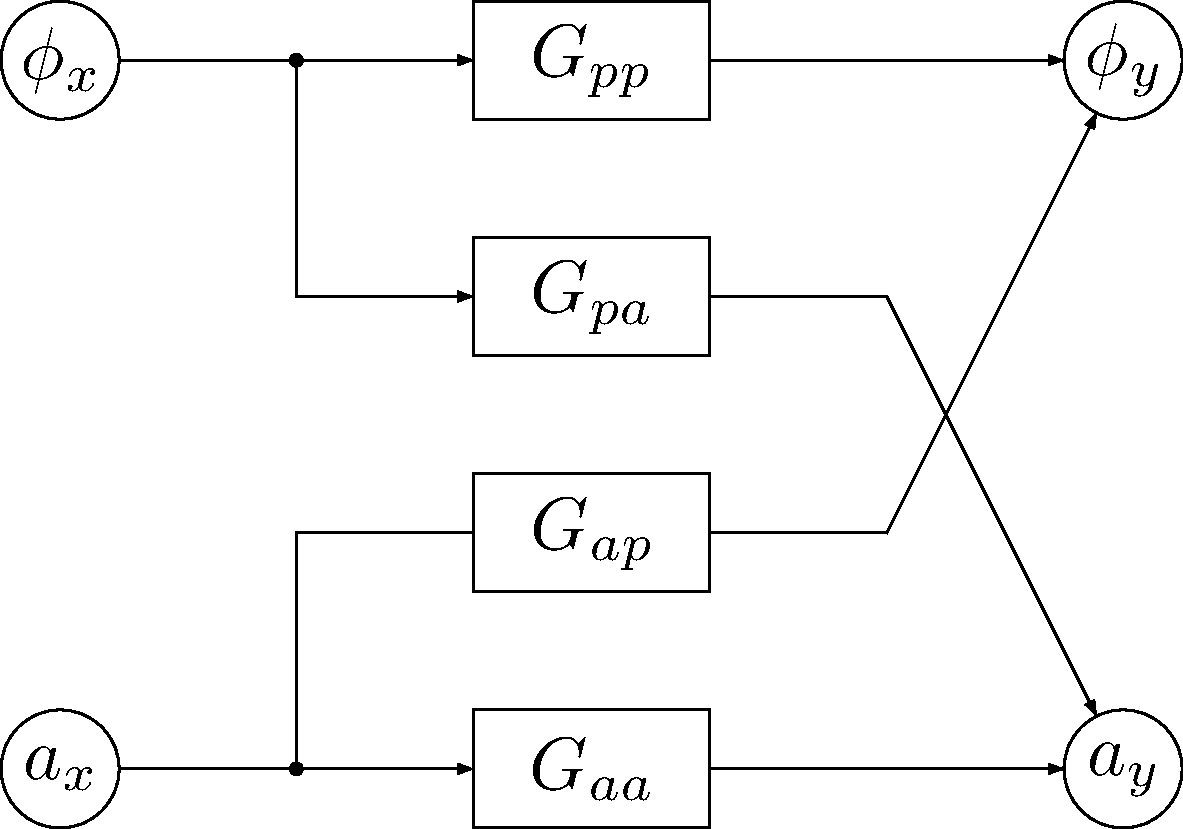
\includegraphics[width=8cm,clip]{figs/Pedersen_Model.pdf}
        \caption{Pedersen Model}
        \label{fig:PM}
    \end{center}
\end{figure}
%

これらの4つの変調伝達関数を求めるのだが、最初は、入力信号の振幅のみが$a_x(t)$で変調された場合を考える。このとき、入力信号$x(t)$は次のようにあらわせる。
%
\begin{equation}
    x(t) = \Re[\hat{X}\{1 + a_x(t)\}e^{j\omega_c t}]
    \label{eq:in_am_sig1}
\end{equation}
%
この入力信号がシステムの伝達関数$H(s)$を通じて出力される信号$y(t)$は$a_x(t)$によって振幅と位相が変調され次のようにあらわせる。
%
\begin{equation}
    y(t) = \Re[\hat{Y}\{1 + a_{y,a}(t)\}e^{j(\omega_c t + \phi_0 + \phi_{y,a} (t))}]
    \label{eq:out_am_sig1}
\end{equation}
%
次に、入力信号の位相のみが$\phi_x(t)$で変調された信号を考えると、次のようになる。
%
\begin{equation}
    x(t) = \Re\{\hat{X} e^{j(\omega_ct + \phi_x(t))}\}
    \label{eq:in_pm_sig1}
\end{equation}
%
このとき、出力信号は先程と同様に考えると、
%
\begin{equation}
    y(t) = \Re\{\hat{Y}(1+a_{y, p}(t))e^{j(\omega_c t + \phi_0 + \phi_{y, p}(t))}\}
    \label{eq:out_pm_sig1}
\end{equation}
%
このとき、変調伝達関数$G_{aa}(s),\;G_{pp}(s).\;G_{ap}(s),\;G_{pa}(s)$は次のようあらわせる。
%
\begin{equation}
    G_{aa}(s) =  \frac{a_{y, a}(s)}{a_x(s)}\; , \; G_{pp}(s) = \frac{\phi_{y, p}(s)}{\phi_x(s)}, \;
    G_{ap}(s) =  \frac{a_{y, a}(s)}{a_x(s)}\; , \; G_{pa}(s) = \frac{\phi_{y, p}(s)}{\phi_x(s)}
 \label{eq:md_tf}
\end{equation}
%
これら4つの変調伝達関数(modulation transfer function)を求めるため、変調の振幅が十分小さい場合$(a \ll 1, \phi \ll 1)$を考える。

ここで、(\ref{eq:in_am_sig1})は、
%
\begin{equation}
    \begin{split}
        x(t) &= \Re\{\hat{X}(1 + a_x(t))e^{j\omega_c t}\} 
            = \hat{X}(\cos\omega_c t + a_x(t) \cos\omega_c t) \\
            &=  \frac{\hat{X}}{2}\left \{(e^{j\omega_c t}+e^{-j\omega_c t})+a_x(t)(e^{j\omega_c t} + e^{-j\omega_c t}) \right \}
            \label{eq:in_am_sig2}
    \end{split}
\end{equation}
%
$X(s)=\mathcal{L}\{x(t)\},\; a_x(s) = \mathcal{L}\{a_x(s)\}$とし、(\ref{eq:in_am_sig2})をラプラス変換すると、
%
\begin{equation}
    X(s) = \frac{\hat{X}}{2}\left \{\frac{1}{s-j\omega_c}+\frac{1}{s+j\omega_c} + a_x(s - j\omega_c)+a_x(s+j\omega_c) \right \}
    \label{eq:lt_in_sig2}
\end{equation}
%
いま、変調の振幅が十分小さい時、つまり、$a_{y, a}(t) \ll 1,\; \phi_{y, a}(t) \ll 1$の時、二次の微少量を無視すると、(\ref{eq:out_am_sig1})は、
%
\begin{equation}
    \begin{split}
        y(t) &\simeq \Re\left [\hat{Y}\{1 + a_{y, a}(t)\}\{1 + j \phi_{y, a} (t)\}e^{j(\omega_c t +  \phi_0)}\right ] \\ 
        &\simeq\Re{\hat{Y}(1 + a_{y, a}(t)+ j \phi_{y, a} (t))e^{j(\omega_c t +  \phi_0)}} \\ 
        &= \hat{Y}\left \{(1+ a_{y,a}(t))\cos(\omega_c t +  \phi_0) 
        - \phi_{y, a}(t)\sin(\omega_c t +  \phi_0) \right \} \\
        &= \frac{\hat{Y}}{2}\left [\left (1+a_{y,a}(t)\right )\left \{e^{j(\omega_c t 
        + \phi_0)}+e^{-j(\omega_c t+\phi_0)}\right \}
        +j \phi_{y,a}(t)\left \{e^{j(\omega_c t+\phi_0)}-e^{-j(\omega_c t + \phi_0)}\right \} \right ]
        \label{eq:out_sig2}
    \end{split}
\end{equation}
%
同様にして、(\ref{eq:out_sig2})をラプラス変換すると、
%
\begin{multline}
    Y(s) = \frac{\hat{Y}}{2}\biggr [\frac{e^{j\phi_0}}{s-j\omega_c}+\frac{e^{-j\phi_0}}{s+j\omega_c} 
    + e^{j\phi_0}a_{y, a}(s - j\omega_c) + e^{-j\phi_0}a_{y, a}(s+j\omega_c) \\
    + j\left \{e^{j\phi_0}\phi_{y,a}(s-j\omega_c) - e^{-j\phi_0}\phi_{y,a}(s+j\omega_c) \right \} \biggl ]
    \label{eq:lt_out_sig2}
\end{multline}
%
ここで、(\ref{eq:md_tf})より
%
\begin{equation}
    a_{y, a}(s) = G_{aa}(s) a_x(s)\; , \quad \phi_{y, a}(s) = G_{ap}(s)a_x(s)
    \label{eq:gaa_gap}
\end{equation}
%
(\ref{eq:gaa_gap})を(\ref{eq:lt_out_sig2})に代入すると、
%
\begin{multline}
    Y(s) = \frac{\hat{Y}}{2}\biggr [\frac{e^{j\phi_0}}{s-j\omega_c}+\frac{e^{-j\phi_0}}{s+j\omega_c} \\
        + e^{j\phi_0}G_{aa}(s-j\omega_c)a_x(s - j\omega_c) + e^{-j\phi_0}G_{aa}(s+j\omega_c)a_x(s+j\omega_c) \\
        + j\left \{e^{j\phi_0}G_{ap}(s-j\omega_c)a_x(s-j\omega_c) 
        - e^{-j\phi_0}G_{ap}(s+j\omega_c)a_x(s+j\omega_c) \right \} \biggl ]\notag 
\end{multline}
%
したがって、
%
\begin{multline}
    Y(s) = \frac{\hat{Y}}{2}\biggr [\frac{e^{j\phi_0}}{s-j\omega_c}+\frac{e^{-j\phi_0}}{s+j\omega_c} 
    + e^{j\phi_0}\{G_{aa}(s-j\omega_c)+j G_{ap}(s-j\omega_c)\}a_x(s-j\omega_c) \\
    + e^{-j\phi_0}\{G_{aa}(s+j\omega_c)- j G_{ap}(s+j\omega_c)\}a_x(s+j\omega_c)\biggl ]
    \label{eq:lt_out_sig3}
\end{multline}
%
ここで、$Y(s) = H(s) X(s)$より、
%
\begin{equation}
    Y(s) = \frac{\hat{X}}{2} \biggl [\frac{1}{s-j\omega_c}+\frac{1}{s+j\omega_c} + a_x(s - j\omega_c) + a_x(s+j\omega_c)  \biggr ] H(s)
    \label{eq:lt_out_sig4}
\end{equation}
%
(\ref{eq:lt_out_sig3})と(\ref{eq:lt_out_sig4})で、係数を比較すると、
%
\begin{equation} 
    \hat{Y}\left(\frac{e^{j\phi_0}}{s-j\omega_c} + \frac{e^{-j\phi_0}}{s+j\omega_c} \right) =
    \hat{X}\left(\frac{1}{s-j\omega_c} + \frac{1}{s+j\omega_c}  \right) H(s) \\
    \label{eq:coef1}
\end{equation}
%
\begin{equation}
    \begin{split}
        G_{aa}(s-j\omega_c) + j G_{ap}(s-j\omega_c) &= \frac{\hat{X}}{\hat{Y}}e^{-j\phi_0}H(s) \\
        G_{aa}(s+j\omega_c) - j G_{ap}(s+j\omega_c) &= \frac{\hat{X}}{\hat{Y}}e^{j\phi_0}H(s) 
    \end{split}
\end{equation}
%
(\ref{eq:coef1})を整理すると、
%
\begin{equation}
    H(s) = \frac{2\hat{Y}}{\hat{X}}\left\{e^{j\phi_0}(s+j\omega_c)+e^{-j\phi_0}(s-j\omega_c)\right\} s
\end{equation}
%
したがって、
%
\begin{equation}
    \begin{split}
        G_{aa}(s) + j G_{ap}(s) &= \frac{H(s+j\omega_c)}{H(j\omega_c)} \\
        G_{aa}(s) - j G_{ap}(s) &= \frac{H(s-j\omega_c)}{H(-j\omega_c)} \\
    \end{split}
\end{equation}
%
これらより、
%
\begin{equation}
    \begin{split}
        G_{aa}(s) &= \frac{1}{2}\left\{\frac{H(s+j\omega_c)}{H(j\omega_c)} + \frac{H(s-j\omega_c)}{H(-j\omega_c)}\right\} \\
        G_{ap}(s) &= \frac{-j}{2}\left\{\frac{H(s+j\omega_c)}{H(j\omega_c)} - \frac{H(s-j\omega_c)}{H(-j\omega_c)}\right\}
    \end{split}
\end{equation}
%

つぎに、$\phi_x(t) \ll 1$より、(\ref{eq:in_pm_sig1})は、
%
\begin{equation}
    \begin{split}
        x(t) &= \Re\{\hat{X} e^{j(\omega_ct + \phi_x(t))}\} \\
            &\simeq \Re\{\hat{X}(1+j\phi_x(t)) e^{j\omega_c t}\} \\
            &= \hat{X} (\cos\omega_c t - \phi_x(t)\sin\omega_c t ) \\
            &= \frac{\hat{X}}{2}\{(e^{j\omega_c t} + e^{-j\omega_c t}) + j \phi_x(t)(e^{j\omega_c t} - e^{-j\omega_c t})\} 
            \label{eq:in_pm_sig2}
    \end{split}
\end{equation}
%
(\ref{eq:in_pm_sig2})をラプラス変換すると、
%
\begin{equation}
    X(s) = \frac{\hat{X}}{2}\left [\frac{1}{s-j\omega_c}+\frac{1}{s+j\omega_c} 
    + j \left \{\phi_x(s - j\omega_c) - \phi_x(s+j\omega_c)\right \} \right ]
    \label{eq:lt_in_pm_sig2}
\end{equation}
%
(\ref{eq:lt_out_sig2})と同様にして(\ref{eq:out_pm_sig1})もラプラス変換すると、
%
\begin{multline}
    Y(s) = \frac{\hat{Y}}{2}\biggr [\frac{e^{j\phi_0}}{s-j\omega_c}+\frac{e^{-j\phi_0}}{s+j\omega_c} 
        + e^{j\phi_0}a_{y, p}(s - j\omega_c) + e^{-j\phi_0}a_{y, p}(s+j\omega_c) \\
        + j\left \{e^{j\phi_0}\phi_{y,p}(s-j\omega_c) - e^{-j\phi_0}\phi_{y,p}(s+j\omega_c) \right \} \biggl ]
        \label{eq:lt_out_pm_sig2}
\end{multline}
%
ここで、(\ref{eq:md_tf})より
%
\begin{equation}
    \phi_{y, p}(s) = G_{pp}(s){\phi_x(s)}\; , \quad a_{y, p}(s) = G_{pa}(s)\phi_x(s)
    \label{eq:gpp_gpa}
\end{equation}
%
となるので、(\ref{eq:gpp_gpa})を(\ref{eq:lt_out_pm_sig2})に代入して整理すると、
%
\begin{multline}
    Y(s) = \frac{\hat{Y}}{2}\biggr [\frac{e^{j\phi_0}}{s-j\omega_c}+\frac{e^{-j\phi_0}}{s+j\omega_c} 
    + e^{j\phi_0}\{G_{pa}(s-j\omega_c)+j G_{pp}(s-j\omega_c)\}a_x(s-j\omega_c) \\
    + e^{-j\phi_0}\{G_{pa}(s+j\omega_c)- j G_{pp}(s+j\omega_c)\}a_x(s+j\omega_c)\biggl ]
    \label{eq:lt_out_pm_sig3}
\end{multline}
%
ここで、$Y(s) = H(s) X(s)$より、
%
\begin{equation}
    Y(s) = \frac{\hat{X}}{2}\left [\frac{1}{s-j\omega_c}+\frac{1}{s+j\omega_c} 
    + j \left \{\phi_x(s - j\omega_c) - \phi_x(s+j\omega_c)\right \} \right ] H(s)
    \label{eq:lt_out_pm_sig4}
\end{equation}
%
(\ref{eq:lt_out_pm_sig3})と(\ref{eq:lt_out_pm_sig4})で、係数を比較すると、
%
\begin{equation}
    \begin{split}
        G_{pa}(s-j\omega_c) + j G_{pp}(s-j\omega_c) &= j \frac{\hat{X}}{\hat{Y}}e^{-j\phi_0}H(s) \\
        G_{aa}(s+j\omega_c) - j G_{ap}(s+j\omega_c) &= -j \frac{\hat{X}}{\hat{Y}}e^{j\phi_0}H(s) 
    \end{split}
\end{equation}
%
したがって、
%
\begin{equation}
    \begin{split}
        G_{pa}(s) + j G_{pp}(s) &= j \frac{H(s+j\omega_c)}{H(j\omega_c)} \\
        G_{pa}(s) - j G_{pp}(s) &= -j \frac{H(s-j\omega_c)}{H(-j\omega_c)} \\
    \end{split}
\end{equation}
%
これらより、
%
\begin{equation}
    \begin{split}
        G_{pp}(s) &= \frac{1}{2}\left\{\frac{H(s+j\omega_c)}{H(j\omega_c)} + \frac{H(s-j\omega_c)}{H(-j\omega_c)}\right\} \\
        G_{pa}(s) &= \frac{j}{2}\left\{\frac{H(s+j\omega_c)}{H(j\omega_c)} - \frac{H(s-j\omega_c)}{H(-j\omega_c)}\right\}
    \end{split}
\end{equation}
%
以上の結果から、変調伝達関数は以下の様になる。
%
\begin{equation}
    \begin{split}
        G_{aa}(s) &= G_{pp}(s) 
        = \frac{1}{2}\left\{\frac{H(s+j\omega_c)}{H(j\omega_c)} + \frac{H(s-j\omega_c)}{H(-j\omega_c)}\right\} = G_s(s)\\
        G_{ap}(s) &= -G_{pa}(s) 
        = \frac{j}{2}\left\{\frac{H(s+j\omega_c)}{H(j\omega_c)} - \frac{H(s-j\omega_c)}{H(-j\omega_c)}\right\} = G_c(s)
    \end{split}
\end{equation}
%
\begin{thebibliography}{9}
    \bibitem{Pedersen}
    F. Pedersen, Beam Loading Effects in the CERN PS Booster, IEEE Trans. Nucl. Sci. 22, 3, June 1975.
    \bibitem{Ninomiya}
    S. Ninomiya, Beam Loading Effect on RF System in Proton Synchrotrons, KEK Report 89-18 (1989).
    \bibitem{llrf}
    S. Simrock, Z. Geng, Low-Level Radio Frequency Systems, Springer (2022)
    \bibitem{Schilcher}
    T. Schilcher Vector sum control of pulsed accelerating fields in Lorentz force detuned superconducting cavities (1998).
    \bibitem{Wilson}
    P. B. Wilson, High energy electron linacs; application to storage ring RF systems and linear colliders (1987)
\end{thebibliography}
%
%
\end{document}